\chapter{Implementation}
\label{chapter:implementation}
\section{Option Pricing}
\label{section:Option Pricing}
The theoretical models presented in Chapter \ref{chapter:background} attempt to replicate the movements of real-world stock prices. With these predictions, we should be able to better reproduce real option prices than if we assumed a simple constant volatility, as did Black \textit{et al.}

Currently, the two most used methods to computationally price options are known as \emph{finite differences}~\cite{Hull} and \emph{Monte Carlo}~\cite{Glasserman}.

The finite differences method is an extremely fast procedure when used to price either European or American-type options, making it very appealing in these circumstances. However, when applied to other option types whose value depends on the stock prices until maturity (e.g. Asian options), the algorithm becomes very slow, rendering it almost useless.
The implementation of both Heston and SABR models (presented before) using finite differences can nonetheless be found in deGraaf~\cite{deGraaf}.


With the Monte Carlo algorithm, we begin by simulating a very large number of stock price paths (e.g. 100,000 simulations). The option's payoff is then calculated for each of these simulated paths and averaged, providing a fairly good estimate of the option's value. This algorithm can be easily adapted to price exotic options, making it very attractive in such cases.
In the past, simulating all the stock price paths took prohibitively long computation times and this method was often discarded for this reason. However, with the recent advancements in computer hardware and new algorithmic developments, such as GPU implementation, this shortcoming has been, to some extent, solved, making the Monte Carlo algorithm quite popular in the present.
For these reasons, the Monte Carlo method will be used for the analysis of the models introduced in Chapter \ref{chapter:background}.


\subsection{Simulating stock prices}
\label{subsection:Simulating stock prices}
As stated, to implement the Monte Carlo algorithm, one needs to simulate stock price paths. However, by analyzing eq.\eqref{GBM}, we can see that the stock prices depend on a Brownian motion process which, due to its self-similarity, is not differentiable~\cite{Mikosch}. It follows that stock price paths can never be exactly simulated. Despite this, we can approximate the movement of stock price paths by discretizing the Brownian motion process in time, thus avoiding its self-similarity problem. We now introduce two of the most common discretization procedures.

\subsubsection{Euler–Maruyama discretization}
One of the simplest and most used discretization methods is known as \emph{Euler–Maruyama discretization}, and can be applied to stochastic differential equations of the type
\begin{equation}\label{SDE}
dX(t)=a(X(t))dt+b(X(t))dW(t),
\end{equation}
\noindent where $a(X(t))$ and $b(X(t))$ are some given functions of $X(t)$ and $\{W(t),\ t>0\}$ defines a one-dimensional Brownian motion process.
To apply this discretization, we begin by partitioning the time interval $[0,T]$ into $N$ subintervals of width $\Delta t=T/N$ and then iteratively define
\begin{equation}
X_{n+1}=X_n+a(X_n)\Delta t+b(X_n)\Delta W_n,\ \ \ n=1,\ldots,N,
\end{equation}
\noindent where $\Delta W_n=W_{t+\Delta t}-W_{t}$.
Using the known properties of Brownian motion processes, it can be shown that $\Delta W_n\sim \sqrt{\Delta t}Z$, where $Z\sim N(0,1)$ defines a standard normal distribution.

Applying this discretization to the Geometric Brownian motion followed by stock price paths, as seen in eq.\eqref{GBM}, we arrive at
\begin{equation}
S(t+\Delta t)=S(t)+rS(t)\Delta t+\sigma(S(t),t)S(t)\sqrt{\Delta t}Z.
\end{equation}

Due to its simplicity, the Euler–Maruyama discretization method is the most common in the simulation of stock price paths whenever we have constant or deterministic volatilities.


\subsubsection{Milstein Discretization}
For stochastic volatility models, such as Heston and SABR, where the volatility itself follows a stochastic process, the Euler–Maruyama discretization may not be sufficiently accurate. In these cases, we can apply the more precise Milstein method~\cite{Milstein}, defined as
\begin{equation}
X_{n+1}=X_n+a(X_n)\Delta t+b(X_n)\Delta W_n+\frac{1}{2}b(X_n)b'(X_n)((\Delta W_n)^2-\Delta t),
\end{equation}
\noindent where $b'(X_n)$ denotes the derivative of $b(X_n)$ w.r.t. $X_n$. Note that when $b'(X_n)=0$, the Milstein method degenerates to the simpler Euler–Maruyama discretization. This discretization should be applied not only to the stock price process but also to the stochastic volatility.

Applying this discretization to the Heston model produces
\begin{equation}
S(t+\Delta t)=S(t)+rS(t)\Delta t+S(t)\sqrt{\nu(t)}\sqrt{\Delta t}Z_1+\frac{1}{2}\nu(t)S(t)\Delta t(Z_1^2-1),
\end{equation}
\begin{equation}
\nu(t+\Delta t)=\nu(t)+\kappa(\overline{\nu}-\nu(t))\Delta t+\eta\sqrt{\nu(t)\Delta t}Z_2+\frac{\eta^2}{4}\Delta t(Z_2^2-1),
\end{equation}
\noindent where $Z_1$ and $Z_2$ are two normal random variables with a correlation of $\rho$.


Applying the Milstein discretization to the SABR model results in
\begin{equation}
\begin{split}
S(t+\Delta t)=&S(t)+rS(t)\Delta t+e^{-r(T-t)(1-\beta)}\sigma(t)S^\beta(t)\sqrt{\Delta t}Z_1+\\
&+\frac{\beta}{2}e^{-2r(T-t)(1-\beta)}\sigma^2(t)S^{2\beta-1}(t)\Delta t(Z_1^2-1),
\end{split}
\end{equation}
\begin{equation}
\sigma(t+\Delta t)=\sigma(t)+\nu\sigma(t)\sqrt{\Delta t}Z_2+\frac{\nu^2}{2}\sigma(t)\Delta t(Z_2^2-1),
\end{equation}
\noindent where again $Z_1$ and $Z_2$ are two normal random variables with a correlation of $\rho$.

In both models we need to generate the two correlated normal variables, $Z_1$ and $Z_2$, which we can easily produce from
\begin{equation}\label{normcorr}
\begin{split}
&Z_1\sim N(0,1);\\
&Z_2=\rho Z_1+\sqrt{1-\rho^2}Y,
\end{split}
\end{equation}
\noindent where $Y\sim N(0,1)$ is uncorrelated with $Z_1$.

Because it is more precise, the Milstein method will be used in the implementation of both Heston and SABR stochastic volatility models. The simpler Euler–Maruyama discretization will be assumed for both constant and Dupire's local volatility.

It is important to note that, the smaller our subintervals $\Delta t$ are, the better is the approximation done when discretizing the Brownian motion process. However, by decreasing $\Delta t$ we increase the number of intervals and with it the number of calculations required to obtain a stock price path. This compromise between computation time and precision must be handled appropriately.
In \autoref{fig:Steps} we can see how smaller subintervals better resemble a true GBM process, whereas if they become too large this resemblance practically vanishes.
\begin{figure}[!htb]
    \centering
      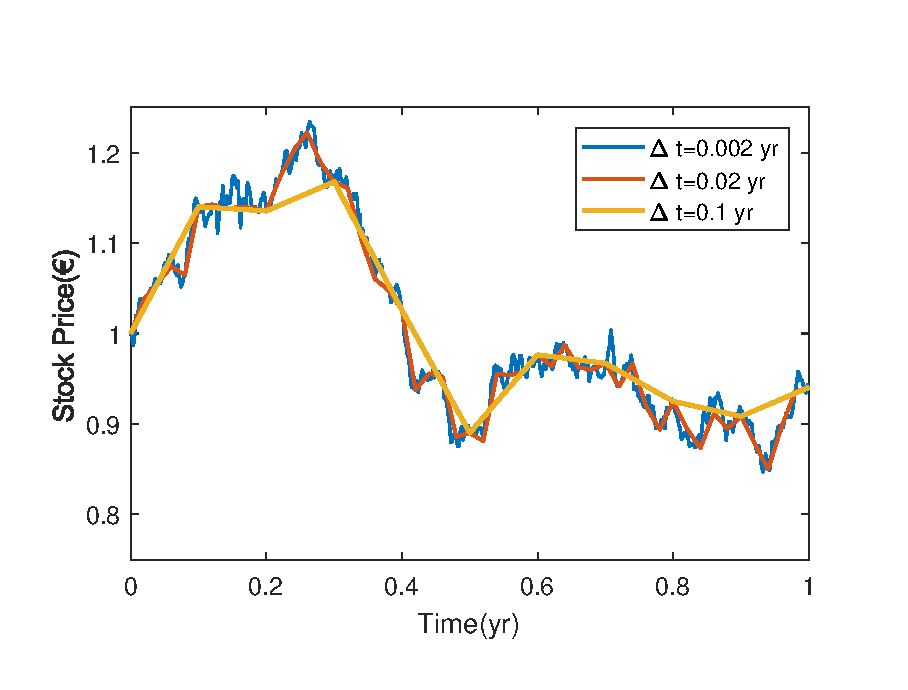
\includegraphics[width=.65\columnwidth]{Steps.eps}
      \caption[Effect of the subinterval size on the GBM discretization]{Effect of the subinterval size on the GBM discretization with maturity $T=\SI{1}{\year}$, interest rate $r=\SI{0.01}{\per\year}$, volatility $\sigma=\SI{0.1}{\year\tothe{-1/2}}$ and initial stock price $S_0=\SI{1}{\EUR}$. The subinterval size selected was $\Delta t=\SI{0.002}{\year}$, $\Delta t=\SI{0.02}{\year}$ and $\Delta t=\SI{0.1}{\year}$ for the blue, red and orange plot lines, respectively. To emphasize this effect, the underlying Brownian Motion $W(t)$ used to generate all three paths was the same.}\label{fig:Steps}
    \end{figure}

\subsection{Pricing options from simulations}
\label{subsection:Pricing options from simulations}
To price options using the Monte Carlo algorithm, we generate $M$ paths by recursively calculating $\{S_i(t),\ \ i=1,\ldots,M\}$, using either of the discretization methods described before.

When the stock price at the maturity, $S_i(T)$, is obtained for all paths, the option's payoff for each path is calculated using eqs.\eqref{callput}-\eqref{barrier}. We then average all these results and discount them back to the present, obtaining the option's value
\begin{equation}\label{mcpricer}
\begin{split}
&C(K,T)=e^{-rT}\frac{1}{M}\sum_{i=1}^M\text{Payoff}_{call}(K,T);\\
&P(K,T)=e^{-rT}\frac{1}{M}\sum_{i=1}^M\text{Payoff}_{put}(K,T),
\end{split}
\end{equation}
\noindent where $\text{Payoff}_{\cdot}(K,T)$ denotes the payoff function of the chosen option type (e.g. European, Barrier, ...).
 

Despite its versatility, the Monte Carlo method can be a very noisy estimator for the price of options, in particular for options with very high strike prices. To understand this problem, notice that the payoff function of European options is zero for stocks below the strike. If we have a very large strike, very few of the simulated paths will actually cross the strike at maturity and contribute to the calculation of the option's price (all the other paths will contribute with a payoff of zero). The averaging procedure shown in eq.\eqref{mcpricer} will therefore be performed on an extremely small subset of paths, which will be noisy.
We could counter this effect by simulating a larger and larger number of paths, so that we always have a significant number of paths above the strike, contributing to the option's price, though this comes at the cost of increased computation times.
Furthermore, on the limit, there will always be a strike high enough that none of the simulated paths reach it, meaning that the option's value for that simulation would be zero. This does not hold in real life, since there is always a positive price for any option, even for extremely high strikes.


\section{Surface Interpolation (Dupire)}
To apply Dupire's local volatility model, as shown in eq.\eqref{dupire2}, we need to generate the implied volatility surface from the market data. Because we only have data for a finite set of maturities and strikes, the implied volatility surface must be obtained by some form of interpolation and extrapolation. From this interpolated surface we must also calculate the gradients needed for the local volatility formula.

Since the data we have is not evenly distributed (e.g. we have strikes $K=0.5$, $0.75$, $0.9$ and $1$, which have different intervals between them), we must choose an interpolation algorithm appropriately. 
 
One possible method is known as \emph{Delaunay triangulation}~\cite{Isaac}. In short, assuming in 2-dimensional data, this interpolation algorithm generates a triangulation between points $P_1$, $P_2$ and $P_3$ if the circumscribed circle of these points contains no other points $P_j$ inside. A scheme of this interpolation method is shown in \autoref{fig:Delaunay}.

\begin{figure}[!htb]
    \centering
      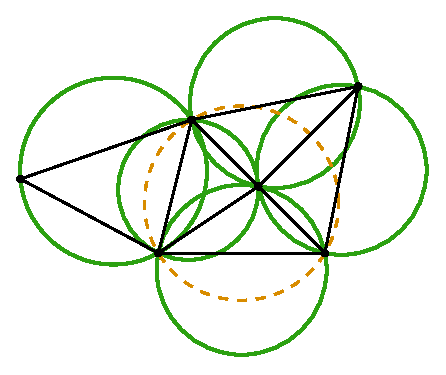
\includegraphics[width=.4\columnwidth]{Delaunay.eps}
      \caption[Example of a Delaunay triangulation, where we connect the points for which the circumscribed circles don't contain any other points inside. A circle for which this property does not hold is also represented, though no triangulation is possible in this case.]{Example of a Delaunay triangulation, where we connect the points for which the circumscribed circles (green) don't contain any other points inside. A circle for which this property does not hold (orange dashed) is also represented, though no triangulation is possible in this case.\\{\small Source: \url{https://www.ti.inf.ethz.ch/ew/Lehre/CG13/lecture/Chapter\%206.pdf}}}\label{fig:Delaunay}
    \end{figure}

 We can easily adapt this algorithm to 3-dimensions (as is the case of our data), using spheres instead of circles.
The resulting interpolated surface will simply be a set of merged triangles. Though this is usually a good approximation, it will produce wrong results when calculating the second derivatives used in the local volatility formula. If we used the first version of Dupire's formula, shown in eq.\eqref{dupire}, where this value is in the denominator, the resulting local volatility surface would become highly unrealistic. However, because the formula in eq.\eqref{dupire2}, which we will use, is not so sensitive to this value, no significant problems are expected.

The function \emph{scatteredInterpolant}, implemented in MATLAB, applies this Delaunay triangulation to a set of scattered data, and will therefore be used in the implied volatility surface generation.



 
\section{Model Calibration (Heston and SABR)}
\label{section:Model Calibration}
Both SABR and Heston stochastic volatility models contain variables that need to be calibrated in order to appropriately replicate market option prices.


Calibrating the models' parameters means finding the optimal values for these parameters such that the difference between the prices of real market options and options priced under the models' assumptions is minimized. This difference should be measured with a cost function such as
\begin{equation}
\mathrm{Cost}(\theta)=\sum_{i=1}^n\sum_{j=1}^mw_{i,j}\left(C_{\mathrm{market}}(T_i,K_j)-C_{\mathrm{model}}(\theta;T_i,K_j)\right)^2,
\end{equation}
\noindent where we denote $\theta$ as the model's parameter set, $w_i$ corresponds to some weight function and where $C_{\mathrm{model}}(\cdot)$ and $C_{\mathrm{market}}(\cdot)$ denote the model and market option prices, respectively, for maturities $T_i,(i=1,\ldots,n)$ and strikes $K_j,(j=1,\ldots,m)$.

Because we are modeling volatilities, and because implied volatilities are more sensitive to slight changes in the parameters, it is more appropriate to use a cost function based on the implied volatility instead of the price, such as
\begin{equation}\label{cost}
\boxed{\mathrm{Cost}(\theta)=\sum_{i=1}^n\sum_{j=1}^mw_{i,j}\left(\sigma_{imp,\mathrm{mkt}}(T_i,K_j)-\sigma_{imp,\mathrm{mdl}}(\theta;T_i,K_j)\right)^2,}
\end{equation}
\noindent where $\sigma_{imp,\mathrm{mkt}}(\cdot)$ and $\sigma_{imp,\mathrm{mdl}}(\cdot)$ correspond to the real-market and model implied volatilities, respectively, for maturities $T_i,(i=1,\ldots,n)$ and strikes $K_j,(j=1,\ldots,m)$. This cost function will be used in the calibration procedure, for the reason stated before.

\hl{consider other weight functions?}


The weight function $w_{i,j}$ should be chosen such that higher weights are given to options with strikes closer to the current stock price $S_0$, because these points have a higher influence in the shape of the volatility smile than the others.
One example of such a function is
\begin{equation}\label{weight}
w_{i,j}=\left(1-\left|1-\frac{K_j}{S_0}\right|\right)^2,
\end{equation}
\noindent where we assume strikes are restricted to $K<2S_0$.
This function is represented in \autoref{fig:weights}.
    
\begin{figure}[!htb]
  \begin{minipage}[b]{0.65\linewidth}
    \centering
    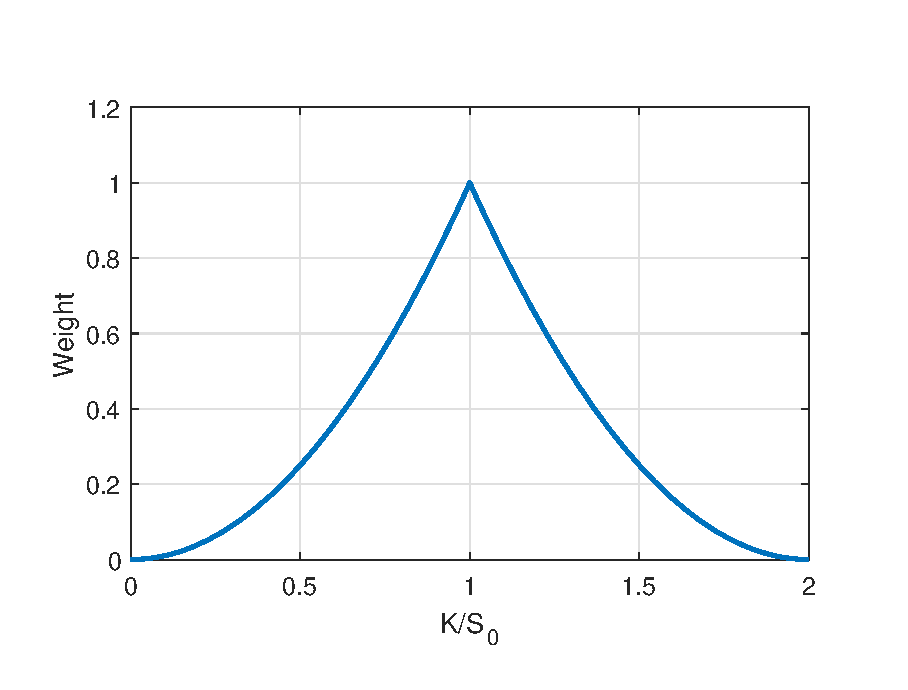
\includegraphics[width=\linewidth]{Weight.eps}
  \end{minipage}%
  \begin{minipage}[b]{0.30\linewidth}
    \centering
    \renewcommand{\arraystretch}{1.1}
\begin{tabular}{@{}lr@{}}
\toprule
$K/S_0$ & Weight \\ \midrule
0.50  & 0.2500 \\
0.75  & 0.5625 \\
0.90  & 0.8100 \\
1.00  & 1.0000 \\
1.10  & 0.8100 \\
1.25  & 0.5625 \\ 
1.50  & 0.2500 \\\bottomrule
\end{tabular}
    \vspace{5em}
  \end{minipage}
\caption[Weight function plot and significant weight values]{Weight function plot and significant weight values}\label{fig:weights}
\end{figure}    
    
\noindent As we can see, the maximum weight value is given to the point where the strike equals the initial stock price ($K=S_0$) and less weight is given for points farther from this value.

To obtain the value of the cost function for a given set of parameters, we need to calculate $m\times n$ model option prices (see eq.\eqref{cost}). We could achieve this by implementing the Monte Carlo method with the discretization procedures described before.
Because we want to calibrate the model's parameters, a large number of instances of the cost function will have to be executed for our optimization algorithms to converge to an optimal solution.
Thus, it can be seen that a very great number of Monte Carlo pricers will have to be executed. For this reason, even with GPU implementation and recent hardware, using Monte Carlo to calibrate the model's parameters will become prohibitively slow. We could reduce the computation time by limiting the number of simulated paths, but this would introduce a high amount of noise in the prices, making the optimization procedure nearly impossible.
Thus, we can conclude that though the Monte Carlo algorithm is very useful to price a small amount of options, it is nearly useless in the calibration procedures required to use both the Heston and SABR models.


We must also mention the fact that, while volatility models are commonplace in finance, investors use different models with different parameters to price their options. This means that even if our calibrated model perfectly fits market data at a given time, after a while the prices will change and the calibration will become outdated. Therefore, a frequent recalibration of the parameters is required which demands fast calibration methods to be employed.


Fortunately, as mentioned, both Heston and SABR have closed-form solutions, shown in eqs. \eqref{CH}, \eqref{sabr} and \eqref{dynsabr}, that we can use to directly price the options with each model's parameters, without the need to run the slow Monte Carlo pricer. The optimization algorithms should then converge much faster to the optimal solution for the model's parameters.





\subsection{Optimization Algorithms}
There are several possible methods to find the parameter set that minimizes the cost function shown in eq.\eqref{cost}.
Our main concern when choosing the best algorithms for calibration is the nonlinearity of the cost function. This is problematic because several local minima might exist and an unsuitable algorithm may get stuck in these points, causing the globally optimal solution to not be found.

With this issue in mind, we selected a powerful algorithm known as \emph{CMA-ES}~\cite{Hansen2} (short for Covariance Matrix Adaptation Evolution Strategy), which we will summarize below. It should be noted that we will only provide a general idea of how this optimizer works. For detailed descriptions, the original source should be consulted.

The optimization algorithm will search the $D$-dimensional sample space ($D$ corresponds to the number of parameters of each model), for the optimal solution. Each point in this space corresponds to a possible set of parameters, $\theta$.




\subsubsection{CMA-ES Optimizer}
The CMA-ES optimizer belongs to the class of evolutionary algorithms. These methods are based on the principle of biological evolution: at each iteration (generation), new candidate solutions (individuals) are generated from a given random distribution (mutation) obtained using the data (genes) of the previous solutions (parents). Of these newly generated solutions (individuals), we select the ones where the cost function is minimized (with the best fitness) to generate the candidate solutions of the next iterations (to become the parents of the next generation) and we reject the others.



As for the CMA-ES in particular, the algorithm takes $\lambda$ samples from a multivariate normal distribution in the $D$-dimensional sample space
\begin{equation}
N(\mathbf{x;m,C})=\frac{1}{\sqrt{(2\pi)^D|\mathrm{det}\mathbf{C}|}}\mathrm{exp}\left(-\frac{1}{2}(\mathbf{x}-\mathbf{m})^T\mathbf{C}^{-1}(\mathbf{x}-\mathbf{m})\right),
\end{equation}
\noindent where $\mathbf{m}$ and $\mathbf{C}$ correspond to the distribution's mean vector and covariance matrix.
These $\lambda$ samples are our candidate solutions.

We classify each of these points according to their fitness (i.e. the cost function's value for a given point). We then select the $\mu$ samples with the lowest cost and discard the others. These new points will be the parents of the next generation, i.e. they will be used to generate the new mean and covariance matrix for the normal distribution.



At each iteration, the new mean is produced from a weighted average of the points, with the weights proportional to each point's fitness.
The method for the covariance matrix update is rather complex and depends not only on the $\mu$ best samples but also on the values of the covariance matrices used in previous iterations. All the basic equations required for the implementation of this optimizer can be found in Appendix \ref{chapter:CMAESAlg}. For a more detailed explanation, as well as other aspects of the algorithm, see Hansen \cite{Hansen}.

These sampling-classification-adaptation steps are repeated until some stopping criterion is met, such as a fixed number of iterations or an minimum error threshold.
When the stopping criterion is met, the mean vector of the last iteration is assumed as the optimal parameter vector.


The number of candidate solutions generated at each step, $\lambda$, and the ones that remain after classification, $\mu$, can be chosen arbitrarily, but an adequate heuristic is to choose $\lambda=\left\lfloor4+3\log D\right\rfloor+1$ and $\mu=\left\lfloor\lambda/2\right\rfloor+1$.

This procedure is summarized in Algorithm \ref{CMAES}.

\begin{algorithm}[H]\label{CMAES}
\DontPrintSemicolon
Define mean vector $\mathbf{m}=\theta_0$\tcc*[r]{Initial guess}
Define covariance matrix $\mathbf{C}=I$\;
\While{Termination criterion not met}{
  Sample $\lambda$ points from multivariate normal distribution $N(\mathbf{x;m,C})$\;
  Calculate the cost for all generated points and keep the $\mu$ best. Discard the rest\;
  Update the mean vector and covariance matrix (using eqs.\eqref{mean} and \eqref{covariance})\;
 }
 Optimal parameters: $\theta^{*}=\mathbf{m}$\;
 \caption{CMA-ES Optimizer}
\end{algorithm}
\

The complexity of the covariance matrix updating process makes the CMA-ES a very robust optimization algorithm, enabling it to find the global optimum of highly nonlinear functions~\cite{DilaoCMA}.
Furthermore, unlike many other optimizers, the CMA-ES is almost non-parametric. It simply requires an starting guess, to generate the starting mean vector, and the algorithm is expected to converge to a global minimum.
As for disadvantages, because we have to generate a set of samples at each iteration, if this generation process is slow, the convergence may stall significantly, particularly when many parameters are used in the model. Other algorithms may perform faster than CMA-ES, but CMA-ES is expected to outperform them in terms of precision.

This optimizer was implemented by Hansen in MATLAB (as well as in other computer languages) as a function named \emph{purecmaes}~\cite{CMAES} and will be used with only very slight changes, to account for the volatility models used used.

